% This is samplepaper.tex, a sample chapter demonstrating the
% LLNCS macro package for Springer Computer Science proceedings;
% Version 2.20 of 2017/10/04
%
\documentclass[runningheads]{llncs}
%
\usepackage{graphicx}
\graphicspath{ {./images/} }
\usepackage[utf8]{inputenc}
\usepackage[spanish,es-nodecimaldot]{babel}
\usepackage[spanish, fixlanguage]{babelbib}
\bibliographystyle{splncs04}
\usepackage{float}
\usepackage{url}
\usepackage{hyperref}
\hypersetup{
	colorlinks=true,
	linkcolor=blue,
	filecolor=magenta,      
	urlcolor=cyan,
}

% Used for displaying a sample figure. If possible, figure files should
% be included in EPS format.
%
% If you use the hyperref package, please uncomment the following line
% to display URLs in blue roman font according to Springer's eBook style:
% \renewcommand\UrlFont{\color{blue}\rmfamily}

\begin{document}
%
\title{Haciendo música con analogías tímbricas.}
\subtitle{Artículo y tesis por Dan Stowell~\cite{stowell_making_2010,stowell_learning_2011}}
%
%\titlerunning{Abbreviated paper title}
% If the paper title is too long for the running head, you can set
% an abbreviated paper title here
%
\author{Saul Ivan Rivas Vega}
%
% First names are abbreviated in the running head.
% If there are more than two authors, 'et al.' is used.
%
\institute{Universidad Nacional Autónoma de México\\
\email{saul.ivan.rivas.vega@comunidad.unam.mx}}
%
\maketitle              % typeset the header of the contribution
%
%
%
\section{Definición del problema}
La síntesis concatenativa ('audio mosaicing') es aquella síntesis de sonido en la que se ocupa una base de conocimiento, en este caso clips de audio, los cuales son concatenados para formar un audio de respuesta dado un audio de consulta. La selección de los clips de audio para la respuesta toma un criterio de emparejamiento a maximizar por cada clip del audio de consulta. Un ejemplo puede verse en la figura~\ref{fig0}. 
\\
\begin{figure}[h!]
	\begin{center}
			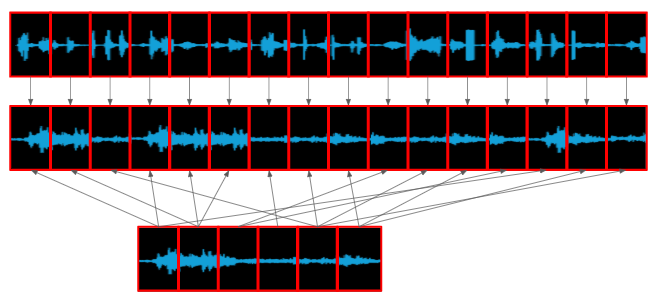
\includegraphics[scale=0.5093]{Captura_000}
		\caption{El audio de consulta (arriba) es segmentado y de la base de datos de segmentos de audio (abajo) se concatenan segmentos para generar un audio de respuesta (en medio).}
		\label{fig0}
	\end{center}
\end{figure}\\
En este trabajo se consideran las características tímbricas para determinar cual es el clip de audio mas adecuado de la base de conocimiento para cada clip del audio de consulta.
En su forma completa un sintetizador concatenativo no solo toma en cuenta las cualidades tímbricas de los sonidos, sino también el ataque o la altura en el caso de sonidos de instrumentos. Sin embargo, en este trabajo se busca generalizar las aplicaciones del sistema por lo que los audios utilizados para los experimentos son distintos principalmente en el timbre. Por lo tanto se excluyen dichas características temporales y de tono.
Otro aspecto tomado en cuenta en el proceso de selección, que se explicará mas adelante, es que únicamente se asigna un segmento de la base de conocimiento por cada segmento de consulta, a diferencia de una extensión a futuro de un sistema completo el cual puede realizar mezclas y modificaciones entre los segmentos mas adecuados de la base de conocimiento.
\paragraph{\textbf{Base de datos de sonidos}} Los audios utilizados en los experimentos consisten en 2 audios musicales con percusiones y 3 ambientales con una frecuencia de muestreo de 44.1 kHz, de los cuales se toman segmentos de 100ms. que tienen una mínima energía arbitraría, el resto son considerados silencios y descartados.\\

Se define en la siguiente sección el espacio tímbrico utilizado en el cual la síntesis concatenativa realizará un mapeo en el que los criterios de selección del segmento de respuesta a cada segmento de consulta sera infiriendo una coordenada en un espacio tímbrico en respuesta a otro.

\section{Características Tímbricas}
No hay una definición universalmente aceptada para el timbre en el cual se puedan medir todos sus componentes, sin embargo en la literatura se llegan a acuerdos frecuentes de algunos de estos. Se llega a considerar al timbre, en sistemas de análisis musical, como la característica del sonido que permite separar una grabación polifónica en pistas agrupadas por similitudes fuera de la intensidad y tono. 

Se consideran atributos que pueden ser medidos a partir de la señal acústica, es incierto aún cuantas dimensiones considerar y si es dependiente del contexto, sin embargo dados los resultados la selección de atributos demuestra ser lo suficientemente robusta en el entendimiento actual del timbre en sonidos no necesariamente musicales.

En cada segmento de 100ms, se realiza un análisis espectral por frecuencias en ventanas de muestreo de 1024 muestras o frames. 
\paragraph{\textbf{Características por muestra:}}
\begin{itemize}
	\item Energía espectral, la cantidad de energía total en la muestra.
	\item Energía espectral por segmentos logarítmicos \begin{itemize}
		\item (50-400Hz, 400-800Hz, 800-1600Hz, 1600-3200Hz, 3200-6400Hz)
		\end{itemize}
	\item Centroide Espectral
	\item Frecuencias de los percentiles espectrales, las frecuencias donde por debajo se concentran el \textbf{95} y \textbf{25} \% de la energía espectral.
	\item Conteo de cruce por cero, cuantas veces en el dominio del tiempo la señal paso por cero.
\end{itemize}
\section{Diseño propuesto}
El sintetizador concatenativo propuesto realiza emparejamientos entre segmentos de audio de una base de datos en respuesta a segmentos de audio de consulta tomando en cuenta puramente la similitud tímbrica comparando 2 metodologías
\begin{itemize}
	\item NN, Vecinos mas cercanos ('Nearest Neighbours'), una ténica de búsqueda clásica en espacios multivariable.
	\item XAMRT, Es la solución propuesta en la tesis y en el artículo, consiste en un árbol asociativo cruzado de regresión. 
\end{itemize}
\paragraph{\textbf{Árbol asociativo cruzado de regresión}} Es un modelo de aprendizaje maquina entrenado para realizar búsquedas/inferencias en un espacio multivariable.\\
El aprendizaje máquina aplica técnicas de estadística y algoritmos que permiten a un sistema adaptar su comportamiento con respecto a los datos.
En nuestro caso el comportamiento que buscamos en el sistema a partir de los datos es el 'Clustering'. El clustering consiste en tomar un conjunto de puntos de datos y agruparlos dado un criterio de similitud, en este caso una similitud tímbrica.
Las restricciones de entrenamiento e inferencia del árbol propuesto implican que el procesamiento del sintetizador sea fuera de linea, es decir se requiere tener acceso a todo el audio de consulta para poder entrenar el modelo y generar una respuesta.
El entrenamiento consiste en una separación recursiva del conjunto de datos en ramificaciones (de ahí el nombre de 'árbol') hasta llegar a una condición de paro arbitraria para evitar que haya una rama o grupo con solo un elemento. En cada ramificación se realiza un proceso estadístico para poder determinar la maximización probabilista de dicha división, es decir que tan probable es que esa sea la mejor división con respecto al audio de consulta. Cada muestra de audio es un punto en el espacio tímbrico el cual se asume Euclidiano y el proceso de ramificación se realiza tanto en el audio de consulta como en el audio de base de datos como se muestra en a figura~\ref{fig1}.
	\begin{figure}[h!]
		\begin{center}
		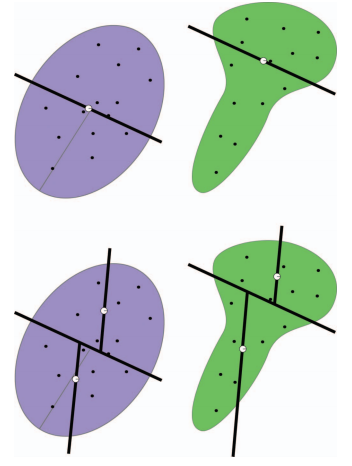
\includegraphics[scale=0.346]{pga_006}
		\caption{Ramificaciones en el conjunto de segmentos del audio de consulta y el audio de base de datos.}
		\label{fig1}
	\end{center}
	\end{figure}\\
Finalmente la inferencia consiste en realizar un recorrido por el espacio tímbrico del audio de consulta y concatenando el correspondiente segmento del audio de base de datos que esta asociado a esa rama en su árbol.

\section{Evaluación y Resultados}
La evaluación con respecto a los resultados individuales requeriría una evaluación con usuarios en pruebas auditivas, sin embargo eso se planteó como trabajo a futuro. Se realizó la evaluación de la eficiencia con la que se realiza el emparejamiento a partir de las probabilidades obtenidas en la creación de las ramificaciones. 
Se consideraron como evaluación la entropía de Shannon por cada segemento.
\begin{equation}
	H(X)=\sum_{i=1}^{|A|} p_i log(p_i)
\end{equation}
De la cual podemos obtener la Eficiencia.
\begin{equation}
Eficiencia(X)=\frac{H(X)}{log(|A|)}
\end{equation}
La mejor eficiencia para la técnica de los vecinos mas cercanos (NN) fue de: \textbf{70.8\%}$\pm$ 4.4, mientras que para el árbol asociativo cruzado fue de: \textbf{84.5\%}$\pm$ 4.8.
\section{Conclusiones}

El algoritmo propuesto permite búsquedas en un espacio multivariable con poca complejidad de consulta y que además es incorporado como parte en un sistema de síntesis concatenativa.
La síntesis concatenativa puede representar una interacción entre 2 espacios discretos con el objetivo de mapear las propiedades de los elementos de un contexto en otro. En este caso de creación musical incorporando una variación tímbrica usando definiciones con base en el entendimiento actual del timbre.
Una versión extendida podría incorporar elementos como el ataque y realizar no solo la concatenación de los segmentos sino que también puedan ser modificados para una mejor eficiencia.\\

Los audios se pueden escuchar de la página oficial del artículo\\
\url{https://archive.org/details/xamrtconcat2010/}\\
O versiones separadas entre audio consulta y audio base en:\\ \url{https://colab.research.google.com/drive/1IiHYFGxtIs9-HPbOl4aYHZvkzsQINf5i?usp=sharing}

\bibliography{main}
\end{document}
